\newpage
\fancyhead[LH]{上海交通大学学位论文}
\fancyhead[RH]{第三章\quad 目标跟踪器搭建}
\section{目标跟踪器搭建}

为了实现路侧单元对车辆的对目标跟踪任务,我们采用了EagerMOT框架。由于缺少合适的路侧目标跟踪数据集,我们在KITTI数据集上对该框架进行了性能测试。

\subsection{EagerMOT原理}

EagerMOT框架结合了互补的2D和3D(例如LiDAR)目标信息,这些信息是从预训练的物体检测器中获得的。框架的总体概述如图\ref{fig18}所示。作为每一帧的输入,首先从预先训练好的检测器中获得一组3D边框检测 $^{3d}D_t$ 和一组2D边框检测 $^{2d}D_t$。然后,融合模块(i) 将来自 2D 和 3D 的检测结果中相同的对象关联起来,(ii)两阶段数据关联模块进行目标关联,并且,该关联基于当前可用的检测结果信息(例如完整的2D+3D信息,仅含2D信息或仅含3D信息),)然后更新跟踪状态和,(iii)最后采用简单的跟踪管理机制初始化或终止轨迹。

这种跟踪方法允许所有检测到的对象与轨迹相关联,即使它们仅在图像域或 3D 传感器中被检测到。这样,当目标被短时间遮挡后可以被恢复。并且当检测器之一漏检时,目标也能保持原有的3D位置。而且重要的是,在目标进入 3D 传感器感知范围之前,这种方法就已经可以在图像域中跟踪远处的物体。 一旦目标进入感应范围,我们对每个轨迹可以顺利地初始化一个 3D 运动模型。

\begin{figure}[htb] 
    \center
    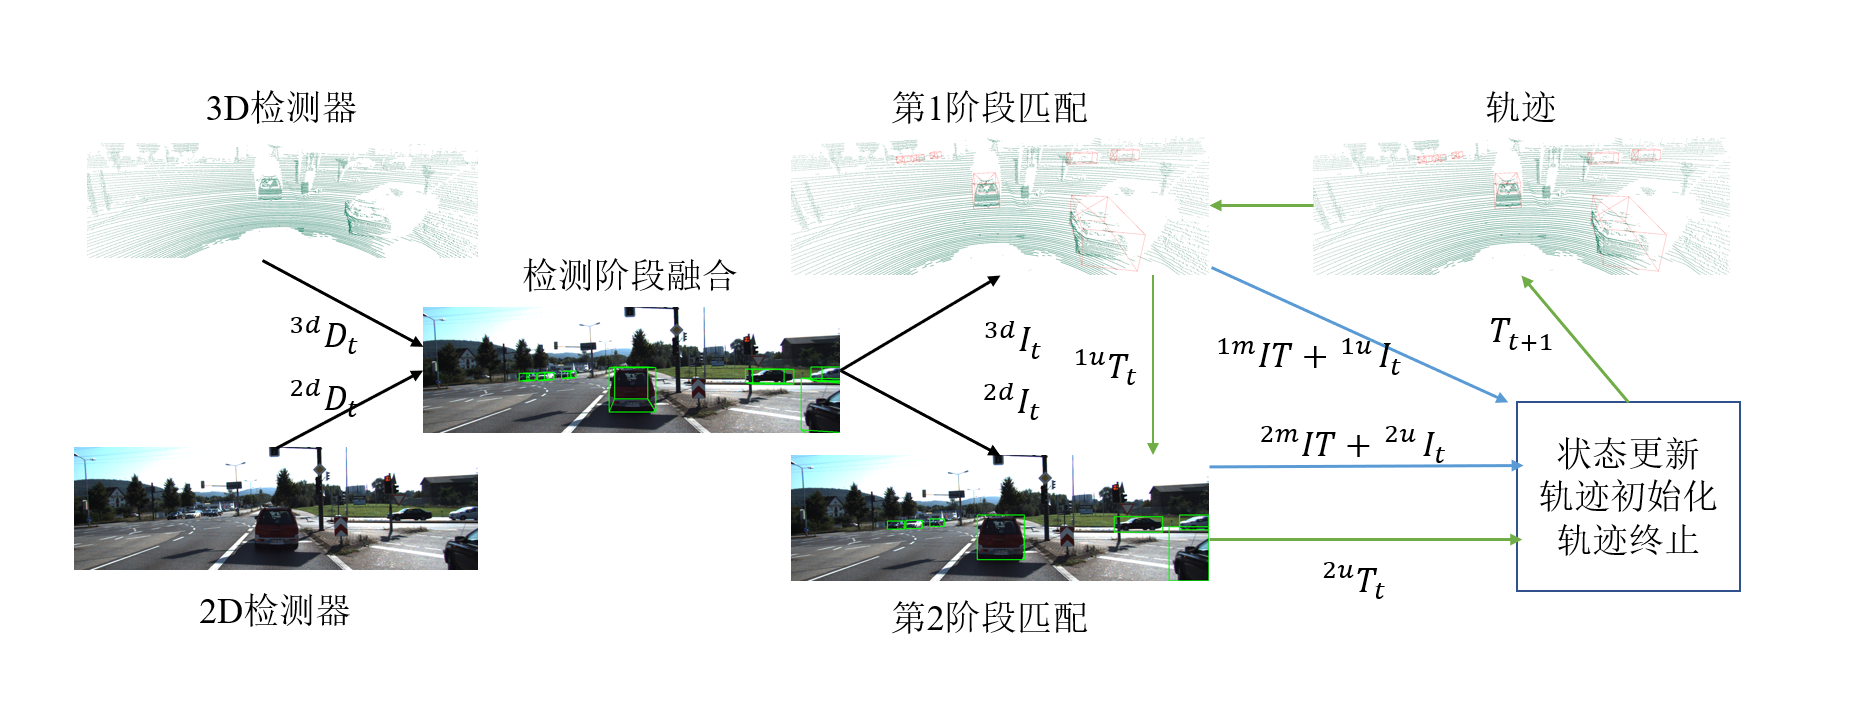
\includegraphics[width=\textwidth]{figure/fig18.png}
    \caption{EagerMOT框架流程图}
    \label{fig18}
\end{figure}

\subsubsection{检测器融合}
\label{sec3.1.1}

获得来自相机的2D视频输入与来自激光雷达3D信息流的检测结果 $^{2d}D_t$ 与 $^{3d}D_t$。设这些来自多传感器的目标的融合结果为$I_t=\{I_t^0,I_t^1,...I_t^n\}$,其中,每一个实例$I_t^i$都对应于现实中的一个目标,它可以同时包含2D与3D的检测信息,也可以仅包含其中一种检测信息。特殊地,定义$^{3D}I_t$为包含了3D检测信息的实例的集合,无论该实例是否包含2D检测信息。类似地,定义$^{2D}I_t$为包含了2D检测信息的实例的集合,无论该实例是否包含3D检测信息

对来自多传感器的检测结果进行数据关联,采用贪心算法,将3D检测结果投影到2D图像域上,计算二者的交比(Intersection of Union)

\begin{equation}
    \text{Intersection of Union} = \frac{\text{Area}_{3D}\cap\text{Area}_{2D}}{\text{Area}_{3D}\cup\text{Area}_{2D}}
\end{equation}
将所有可能的检测配对按照交比进行排序,按照交比从高到低的顺序,当2D与3D检测结果均尚未配对成功,且交比大于预先设置的阈值(threshold)$\theta_{fusion}$时,产生融合实例 $^{both}I_t^i$。以此得到融合的检测实例集合$^{both}I_t$ 。其中,每个实例 包含了来自2D检测器的2D 边界框(bounding box)与来自3D检测器的3D位置与3D边界框,因此 也属于两个单模态检测实例集合$^{3D}I_t$与$^{2D}I_t$,即$^{both}I_t\in^{3D}I_t$且$^{both}I_t\in^{2D}I_t$

将剩下的未匹配的检测结果$^{3D}I_t^i$与$^{2D}I_t^i$作为部分观测结果(partial observation)加入检测实例集合 中与对应的 中。

上面的思路虽然简单,但是过去的经验证明了它的鲁棒性。

\subsubsection{数据关联}

数据关联分为两阶段进行,在第一阶段进行3D目标的数据关联,将3D检测结果 与已有的3D轨迹 匹配。在第二阶段,在2D图像域进行目标关联,弥补目标遮挡时3D检测器漏检的场景。

\textbf{轨迹参数} 同时包含2D与3D信息的轨迹为 $^{both}I_t$,包含3D信息的轨迹为 ,包含2D信息的轨迹为 $^{2D}I_t$。它们有如下关系:$^{both}I_t\in^{3D}I_t$且$^{both}I_t\in^{2D}I_t$。其中,$^{3D}I_t$额外设置了一个速度参数$v$。

\textbf{一阶段匹配} 首先用3D信息将3D检测结果 $^{3D}I_t$与已有的3D轨迹 $^{3D}T_t$匹配,计算 $^{3D}I_t$与 $^{3D}T_t$间的缩放距离(scaled distance)。缩放距离如下定义

\begin{eqnarray}
    &d(B^i,B^j)=||B^i_\rho-B^j_\rho||*\alpha(B^i,B^j)\\
    &\alpha(B^i,B^j)=2-\cos\langle B_\gamma^i,B_\gamma^j\rangle
\end{eqnarray}
其中, $B_\rho^i=[x,y,z,h,w,l]$是包含了3D位置信息与包围框信息的向量, 表示了包围框相对于地面纵轴的方向。这种缩放距离与传统的欧式距离或马氏距离相比在实验结果中更加鲁棒。

如同\ref{sec3.1.1}中的贪心算法,按照缩放距离从小到大对“目标-轨迹”对进行排序,将匹配最佳且缩放距离小于阈值的“目标-轨迹”对作为成功的配对。输出配对的集合$^{1m}IT_t={{I_t^i,T_t^j},...}$其余未匹配的结果标记为 $^{1u}I_t$与 。此时所有的3D结果,或者成功配对,或者未配对且不参与后续匹配。

\textbf{二阶段匹配} 在图像域用仅有2D信息的实例 $^{2D}I_t\backslash^{both}I_t$与剩下的2D轨迹 $^{1u}T_t\cap^{2D}T_t$匹配。匹配方式与\ref{sec3.1.1}类似,计算目标与轨迹的2D交比,根据交比及阈值$\theta_{2D}$用贪心算法匹配。值得注意的是,轨迹在包含3D信息时,将3D预测框投影到2D图像域作为边界框计算,仅在不含3D信息时,将最后一次记录的2D边界框参与计算。此阶段输出的结果为匹配对$^{2m}IT_t=\{\{I_t^i,T_t^j\},...\}$

\textbf{状态更新} 2D边界框直接采用匹配目标的2D边界框,如果该目标包含2D信息。3D状态则被建模为多元高斯函数,使用线性卡尔曼滤波更新。

\begin{equation}
    X_{update}=X_t+v*dT
\end{equation}
这一步与AB3DMOT框架\cite{weng20203d}完全一致。但当匹配的目标不包含3D信息时,轨迹只通过卡尔曼滤波进行预测步骤以延拓状态。

\subsubsection{轨迹生命周期管理}

这一步与AB3DMOT类似,当一个轨迹在 $Age_{max}$帧没有被匹配后,将被舍弃,未被匹配的新目标会被当作新轨迹加入后续匹配中。但论文考虑到2D检测结果往往比3D检测结果更可信,只有当一个轨迹连续 $Age_{2D}$帧与2D信息匹配成功后,才会被认为是一个可信的新轨迹。

\subsection{评价指标}

衡量一个目标跟踪框架好坏有多种指标,早期常用的是CLEAR MOT\cite{bernardin2008evaluating}指标。近些年HOTA\cite{luiten2021hota}指标成为了各个目标跟踪比赛的主流指标。

\subsubsection{CLEAR MOT指标}

理想追踪器有3个需求:(1)在所有时刻找出正确的物体数量,(2)尽可能精确地估计出每个物体的位置,(3)指派连续的ID,即使有遮挡。

假设在跟踪场景中,某一帧的目标位置信息为$\{o_1,o_2,...,o_n\}$,而跟踪算法给出的目标假设信息(hypothesis)为$\{h_1,h_2,...,h_m\}$。我们需要(1)在h和o之间建立最大可能性连接,这一点往往是给定阈值$\alpha$,当$h$与$o$之间的交比超过$\alpha$时,设定为匹配成功。(2)对于每一个连接,使用位置估计计算误差(3)积累所有的连接误差:没有设定假设h的目标o(Miss),没有对于目标o的假设h(False Positive);同一个目标ID改变(Mismatch)。

最终论文导出了两大指标:MOTA(Multiple Object Tracking Accuracy)与MOTP(Multiple Object Tracking Precision)

MOTA用于衡量跟踪器的准确度:

\begin{equation}
    \text{MOTA}=1-\frac{\Sigma_t(m_t+fp_t+mme_t)}{\Sigma_tg_t}
\end{equation}
其中$m_t$,$fp_t$与$mme_t$分别为丢失(miss),错检(false positive)与ID切换(mismatch)的数量。

MOTP用于衡量跟踪器的精确度:

\begin{equation}
    \text{MOTP}=\frac{\Sigma_{i,t}d_t^i}{\Sigma_tc_t}
\end{equation}
其中$d^i$为匹配的$\{o,h\}$对之间的距离,$c_t$匹配的$\{o,h\}$对的个数。

由于目前流行的还是“检测-跟踪”范式,即检测器输出检测结果,跟踪器只需指出前后两帧间目标的对应关系。因此,跟踪器的精确度主要取决于检测器的精度,MOTP不太能反映跟踪器本身的性能。所以MOTA被广泛采用为首要指标。

\subsubsection{HOTA指标}

MOTA虽然在长时间里被用作跟踪器性能好坏的指标,但是它过于强调检测器的性能。一种极端情况是,检测的性能非常优秀,但是所有检测到的目标不做跟踪,而是全部分配一个相同的track id,此时的MOTA会非常高,因为$mme=0$。

HOTA指标则综合考虑了不同匹配阈值$\alpha$下的检测精度与关联精度

\begin{equation}
    \mathrm{HOTA}=\int_{0}^{1} HOTA_{\alpha} \mathrm{d} \alpha \approx \frac{1}{19} \sum_{\alpha \in\left\{\begin{array}{c}
        0.05,0.1, \ldots \\
        0.9,0.95
        \end{array}\right\}} HOTA_{\alpha}
\end{equation}
其中$HOTA_{\alpha}$为阈值$\alpha$下的HOTA指标
\begin{eqnarray}
    HOTA_{\alpha}
    & =\sqrt{\displaystyle\frac{\Sigma_{c\in{TP}}\mathcal{A}(c)}{|TP|+|FN|+|FP|}}\\
    & =\sqrt{\displaystyle DetA_\alpha\cdot AssA_\alpha}
\end{eqnarray}
其中$DetA_\alpha$与$AssA_\alpha$分别衡量跟踪器的检测精度与匹配准度
\begin{eqnarray}
    DetA_\alpha=\frac{|TP|}{|TP|+|FN|+|FP|}\\
    AssA_\alpha=\frac{1}{|TP|}\Sigma_{c\in{TP}}\mathcal{A}(c)\\
    \mathcal{A}(c)=\frac{|TPA(c)|}{|TPA(c)|+|FNA(c)|+|FPA(c)|}
\end{eqnarray}
TP,FP,FN分别为正确的检测(True Positive),错检(False Positive)和漏检(False Negtive)的数量。对于每一个正确的检测c,类似有正确关联TPAs (True Positive Associations), 错误关联FNAs (False Negative Associations) and 漏关联FPAs (False Positive Associations)等指标。

\subsection{实验结果}

我们下载了论文中提到的检测器与数据集,如表\ref{table3}所示。

\begin{table}[htbp]
    \centering
    \caption{EagerMOT数据集与检测器设置}
    \begin{tabular}{c c}
    \toprule
    框架 & 框架名称 \\
    \midrule
    数据集 & KITTI, NuScenes\\
    2D检测器 & Track-RCNN, MOTSFusion, RCC\\
    3D检测器 & Point-RCNN, Point-GNN\\
    \bottomrule
    \end{tabular}
    \label{table3}
\end{table}

注意到,论文中提到的检测器,其实并非训练好的模型或者权重文件,而是检测器对KITTI数据集评测产生的检测结果。这意味着,如果我们想要使用这些检测器用于其他数据集,需要下载模型重新进行训练。

论文采用了CLEAR-MOT, HOTA, AB3DMOT等指标作为评测标准,在如表\ref{table4}所示的基准测试(benchmark)中进行了评测:

\begin{table}[htbp]
    \centering
    \caption{EagerMOT论文评测的数据集}
    \begin{tabular}{c c}
    \toprule
    数据集 & 划分(split) \\
    \midrule
    KITTI 2D MOT & 测试集 \& 评测集\\
    KITTI 3D MOT & 评测集 \\
    NuSences 3D MOT & 测试集 \& 评测集\\
    \bottomrule
    \end{tabular}
    \label{table4}
\end{table}

我们用MOTSFusion+RCC作为2D检测器,Point-GNN作为3D检测器,HOTA作为评价指标在KITTI数据集的评测集上对car类型目标进行了评测。评测结果如图\ref{table5}

\begin{longtable}{@{\extracolsep{\fill}}cccccccc}
    \caption{EagerMOT评测结果}
    \label{table5}\\
    \toprule
    \makecell{KITTI\\ Sequence} & HOTA & DetA & AssA & DetRe & DetPr & AssRe & AssPr \\
    \midrule
    \endfirsthead

    \text{续表 \thetable}\\
    \toprule
    \makecell{KITTI\\ Sequence} & HOTA & DetA & AssA & DetRe & DetPr & AssRe & AssPr \\
    \midrule
    \endhead

    \bottomrule
    \endfoot

    0002 & 53.711 & 49.066 & 59.081 & 50.789 & 86.084 & 61.606 & 88.639 \\
    0006 & 80.969 & 84.762 & 77.656 & 88.168 & 89.059 & 79.912 & 91.349 \\ 
    0007 & 83.244 & 81.566 & 85.05 & 90.391 & 83.947 & 91.531 & 87.421 \\
    0008 & 76.27 & 81.024 & 71.936 & 84.769 & 85.533 & 74.265 & 87.491 \\
    0010 & 81.261 & 78.375 & 84.384 & 83.929 & 87.868 & 86.242 & 92.934 \\
    0013 & 39.585 & 17.872 & 87.752 & 89.895 & 17.979 & 89.895 & 89.895 \\
    0014 & 77.485 & 75.13 & 80.428 & 81.38 & 83.41 & 85.91 & 87.112 \\
    0016 & 81.565 & 84.502 & 79.052 & 87.761 & 88.077 & 80.403 & 91.35 \\
    0018 & 86.987 & 85.657 & 88.485 & 90.081 & 88.63 & 91.454 & 91.406 \\
    COMBINED & 78.529 & 76.839 & 80.506 & 82.917 & 85.081 & 84.239 & 89.777 \\
\end{longtable}

由于test set的真值(ground truth)储存在KITTI官网的server中,不对外开放,我们无法直接与论文中的结果进行比较,但在val set中得到的评测结果与论文在test set中得到的结果(HOTA 74.39, DetA 75.27, AssA 74.16)差距在合理的范围内,甚至评测指标更高。我们用论文提供的可视化代码生成了视频文件,大部分轨迹连续,且目标切换频率较少。验证了该算法在KITTI数据集上的有效性。

\subsection{本章小节}

本章首先介绍了EagerMOT目标跟踪框架的原理,再介绍了目标跟踪常用的评测方法,最后在KITTI数据集上复现了该框架,并与论文结果进行了对比。